\section{Results}\label{sec:results}
The cross-sectional formulation is validated against two-dimensional (2-D) solid
finite-element homogenization on four examples of increasing complexity: a webbed
\emph{two-cell} tube (isotropic and anisotropic), a \emph{four-cell elliptic} tube at a
thin and a thick wall, the \emph{IEA-22-280-RWT} blade cross-section at $r/R=0.2$ with a
mesh-convergence study, and the \emph{full IEA-22 blade} homogenized at every span
station. Throughout, the equivalent-beam Timoshenko $6\times6$ is written $C^{b}_{ij}$
(the superscript $b$ for \emph{beam}), with the diagonal entries the extension
$C^{b}_{11}$, the transverse shears $C^{b}_{22}$ and $C^{b}_{33}$, the torsion
$C^{b}_{44}$, and the bendings $C^{b}_{55}$ and $C^{b}_{66}$; it is not to be confused
with the direction cosine $C^{ab}_{33}$ of Section~\ref{sec:drill}. The reported error is
$(C_{ij}^{\mathrm{shell}}-C_{ij}^{\mathrm{solid}})/C_{ij}^{\mathrm{solid}}$ on every
nonzero constant, couplings included. The RM shell applies the $\gamma_{23}$-tie of
Section~\ref{sec:mitc} in the thin-wall regime; the tie was verified numerically inert
on the prismatic contour (Section~\ref{sec:mitc}), so no reported number depends on it.
The laminate reference follows the mesh convention: the tube and ellipse contours lie on
the wall \emph{mid-surface} (laminate centred on the line), whereas the airfoil contours
lie on the \emph{outer mold line} (OML) with the laminate stacked inward---the standard
OpenSG blade convention. The distinction is not cosmetic: centring the laminate on the
OML contour pushes half the wall outside the true section, and at $r/R=0.2$ turns the
torsion and flapwise-bending errors from $-2.8\%$ and $+0.9\%$ into $+7.9\%$ and
$+8.0\%$, the spurious stiffening growing to $16\%$ at the thick mid-span walls.

%----------------------------------------------------------------------------------
\subsection{Example 1: webbed two-cell tube}\label{sec:res_two}
A circular tube (mid-wall radius $R=5$~cm, wall $t=4$~mm) with a diametral web forms the
simplest multi-cell section, and the flat web joining the curved skin is precisely the
junction that exposes the drilling treatment (Section~\ref{sec:drill}). Two walls are
considered: an isotropic aluminium wall and a $[-45^\circ]$ single-ply laminate, the
latter activating the extension--twist and shear--bending couplings.
Figure~\ref{fig:twocell} shows the two computed meshes. Table~\ref{tab:two} lists every
nonzero Timoshenko constant for both walls: the RM 6-DOF cross-section reproduces the
2-D solid within $2.2\%$ on every term---including the anisotropic couplings---and the
torsion within $0.5\%$.

\begin{figure}[htbp]\centering
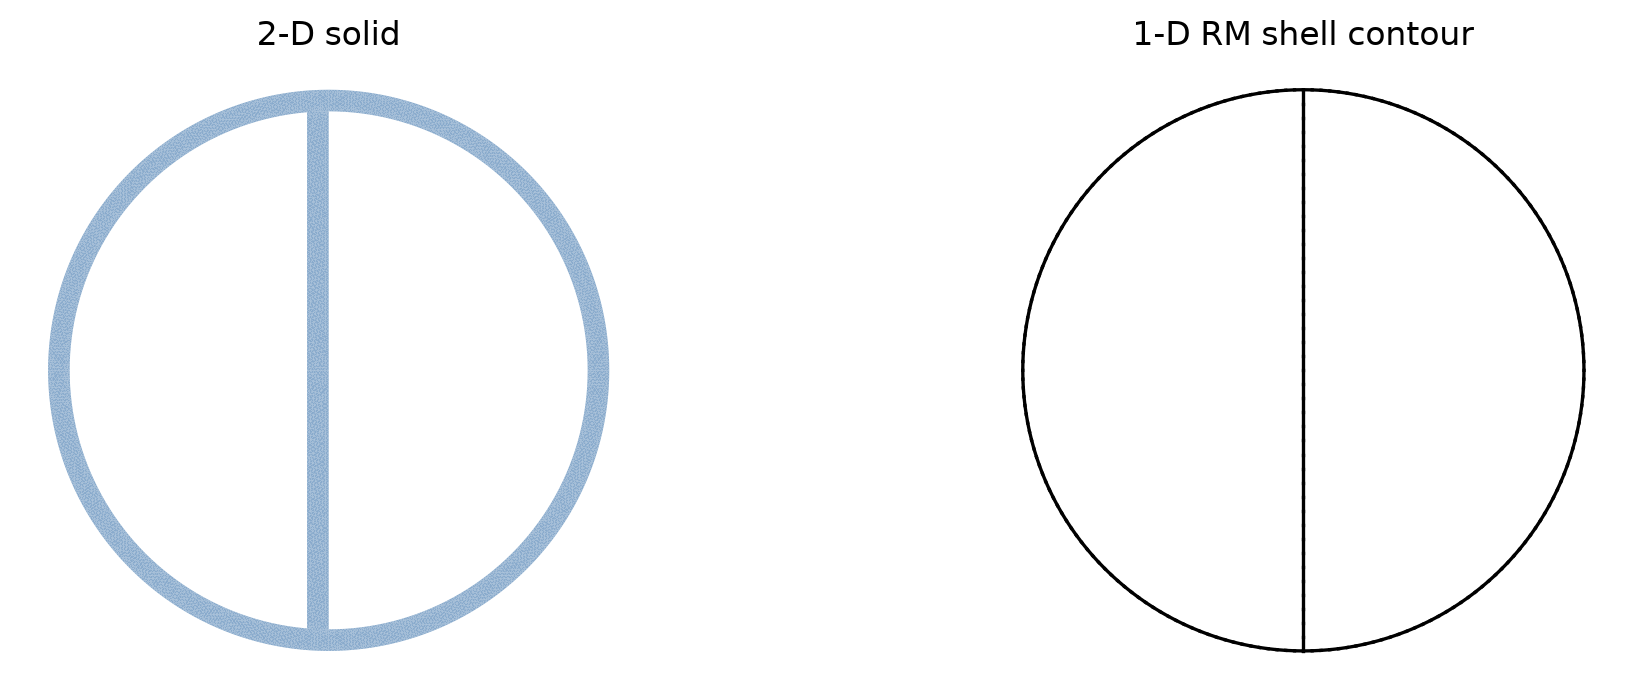
\includegraphics[width=0.6\textwidth]{figures/twocell_mesh.png}
\caption{Webbed two-cell tube: 2-D solid mesh (filled by material) with the 1-D RM shell
mid-surface contour overlaid as the dotted centre reference.}\label{fig:twocell}
\end{figure}

\begin{table}[htpb]
\centering
\small
\caption{Webbed two-cell tube ($R=5$~cm, $t=4$~mm): RM 6-DOF shell vs.\ the 2-D solid, isotropic and $[-45^\circ]$ laminate ($\times10^{7}$).}
\label{tab:two}
\setlength{\tabcolsep}{4.5pt}
\begin{tabular}{l|rrr|rrr}
\hline
 & \multicolumn{3}{c|}{isotropic} & \multicolumn{3}{c}{$[-45^\circ]$} \\
$C^{b}_{ij}$ & solid & shell & \%err & solid & shell & \%err \\
\hline
$C^{b}_{11}$ & $11.3$ & $11.41$ & $+1.0$ & $2.001$ & $2.021$ & $+1.0$ \\
$C^{b}_{13}$ & $\sim\!0$ & $\sim\!0$ & --- & $-0.1198$ & $-0.1223$ & $+2.2$ \\
$C^{b}_{14}$ & $\sim\!0$ & $\sim\!0$ & --- & $-0.02092$ & $-0.02109$ & $+0.8$ \\
$C^{b}_{22}$ & $1.647$ & $1.631$ & $-1.0$ & $0.4488$ & $0.4426$ & $-1.4$ \\
$C^{b}_{25}$ & $\sim\!0$ & $\sim\!0$ & --- & $0.01045$ & $0.01036$ & $-0.8$ \\
$C^{b}_{33}$ & $2.581$ & $2.577$ & $-0.2$ & $0.7335$ & $0.7328$ & $-0.1$ \\
$C^{b}_{36}$ & $\sim\!0$ & $\sim\!0$ & --- & $0.01013$ & $0.01037$ & $+2.4$ \\
$C^{b}_{44}$ & $0.008186$ & $0.008151$ & $-0.4$ & $0.002357$ & $0.002346$ & $-0.5$ \\
$C^{b}_{55}$ & $0.01286$ & $0.01312$ & $+2.0$ & $0.002248$ & $0.002286$ & $+1.7$ \\
$C^{b}_{66}$ & $0.01085$ & $0.01083$ & $-0.2$ & $0.001922$ & $0.001918$ & $-0.2$ \\
\hline
\end{tabular}
\end{table}

Table~\ref{tab:twodrill} isolates the torsion against the five-parameter
drilling-eliminated element of Section~\ref{sec:fivedof}. The two formulations agree on
the classical and shear constants, but the eliminated element mispredicts the torsion
$C^{b}_{44}$ by $+8.3\%$, whereas the 6-DOF element holds it to $-0.4\%$: the Lagrange
constraint recovers the drilling-carried torsional shear that the flat-wall elimination
\eqref{eq:om3} destroys. The correction is not free---on this contour the eliminated
element carries $5$ DOF per node ($1{,}195$ total) against $6$ per node plus one
multiplier per element ($1{,}674$, some $40\%$ more)---but the extra unknowns are what
keep the flat-web shear channel well-posed. This single term is why a multi-cell
section---flat webs joining curved skins---requires the constrained six-parameter model.

\begin{table}[htpb]
\centering
\caption{Two-cell tube torsion $C^{b}_{44}$: the six-parameter drilling-constrained (Lagrange) element against the five-parameter drilling-eliminated element ($\times10^{4}$). The Lagrange constraint recovers the drilling-carried torsional shear that the flat-wall elimination destroys.}
\label{tab:twodrill}
\begin{tabular}{l rr}
\hline
model & $C^{b}_{44}$ & \%err \\
\hline
solid (2-D reference) & $8.186$ & --- \\
RM 6-DOF (Lagrange) & $8.151$ & $-0.4$ \\
RM 5-DOF (eliminated) & $8.863$ & $+8.3$ \\
\hline
\end{tabular}
\end{table}

Figure~\ref{fig:conv2} shows the RM mesh convergence: every diagonal constant is within
$0.6\%$ of its converged value already at $N=40$ circumferential elements and settled to
three figures by $N=160$, so the errors of Table~\ref{tab:two} are model error, not
discretization.

\begin{figure}[htbp]\centering
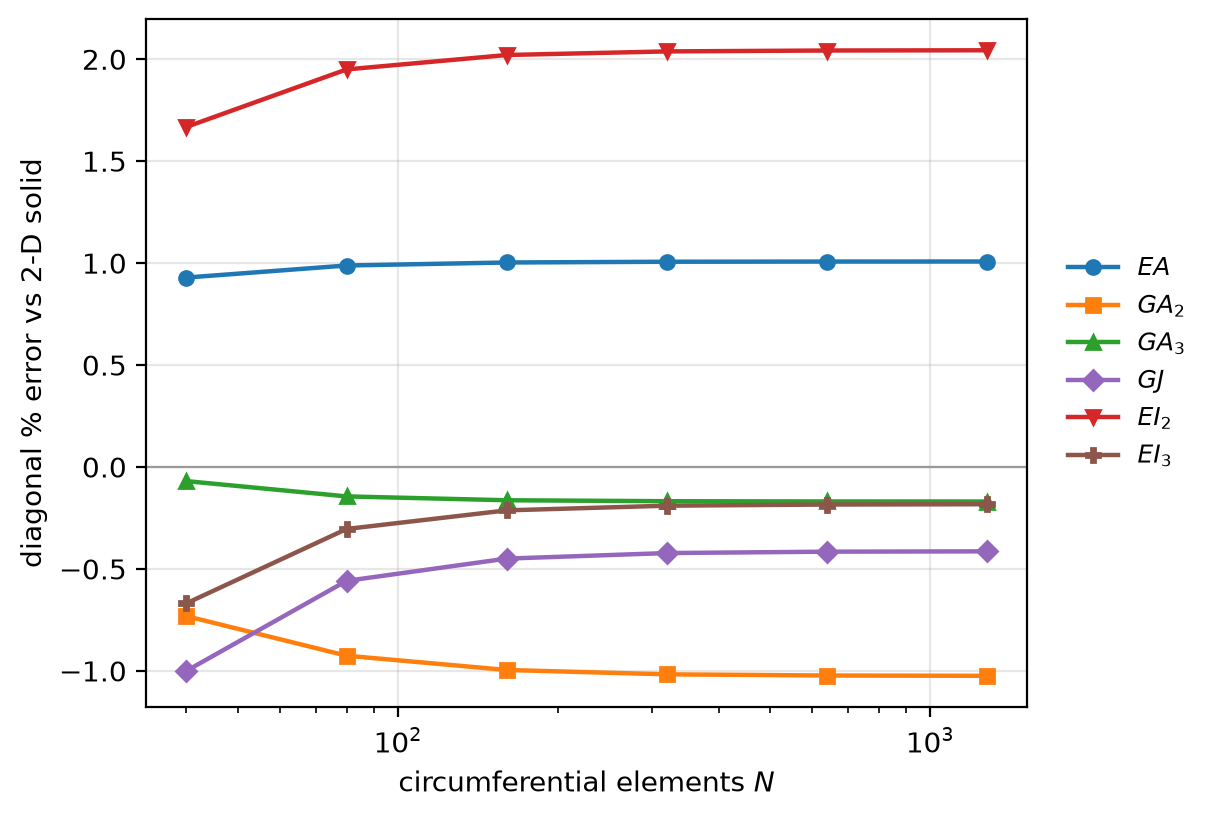
\includegraphics[width=0.62\textwidth]{figures/conv_twocell.png}
\caption{Two-cell tube: RM 6-DOF diagonal \% error vs.\ circumferential element count
$N$ (isotropic wall).}\label{fig:conv2}
\end{figure}

%----------------------------------------------------------------------------------
\subsection{Example 2: elliptic four-cell tube, thin and thick}\label{sec:res_ell}
The elliptic tube (semi-axes $a=1.0$, $b=0.6$~m) with three internal webs is a four-cell
section representative of a multi-web blade box (Figure~\ref{fig:ell4}). It is analysed
at a thin wall ($t/a=0.02$) and a six-times thicker wall ($t/a=0.12$), for the isotropic
and the $[-45^\circ]$ wall, each against a 2-D solid computed independently at that wall.
Tables~\ref{tab:elliso} and~\ref{tab:ellm45} give the term-by-term comparison. The
isotropic section is reproduced within $4.8\%$ (thin) and $3.4\%$ (thick), the torsion
essentially exactly at both walls. The anisotropic section shows one deliberate
exception: at the thin wall the chordwise shear $C^{b}_{22}$, carried almost entirely by
the three off-axis $[-45^\circ]$ webs, is under-predicted by $26\%$---the transverse-shear
limit of a single-director wall on a thin, fully off-axis web---\emph{thickening the wall restores it} to $-0.6\%$, and the remaining diagonal constants
stay within $2.7\%$ at both walls. Only the diagonal constants are tabulated for the
anisotropic section: its sign-odd couplings are reproduced in magnitude but flip sign
against the present hand-generated solid web mesh, whose through-thickness axis convention
differs from the shell's---a mesh-orientation artifact, not a shell-formulation error, and
one the PreVABS solid resolves. The RM cross-section is thus reliable from thin to thick
walls, with the one documented mechanical exception of chordwise shear through thin
fully-anisotropic webs.

\begin{figure}[htbp]\centering
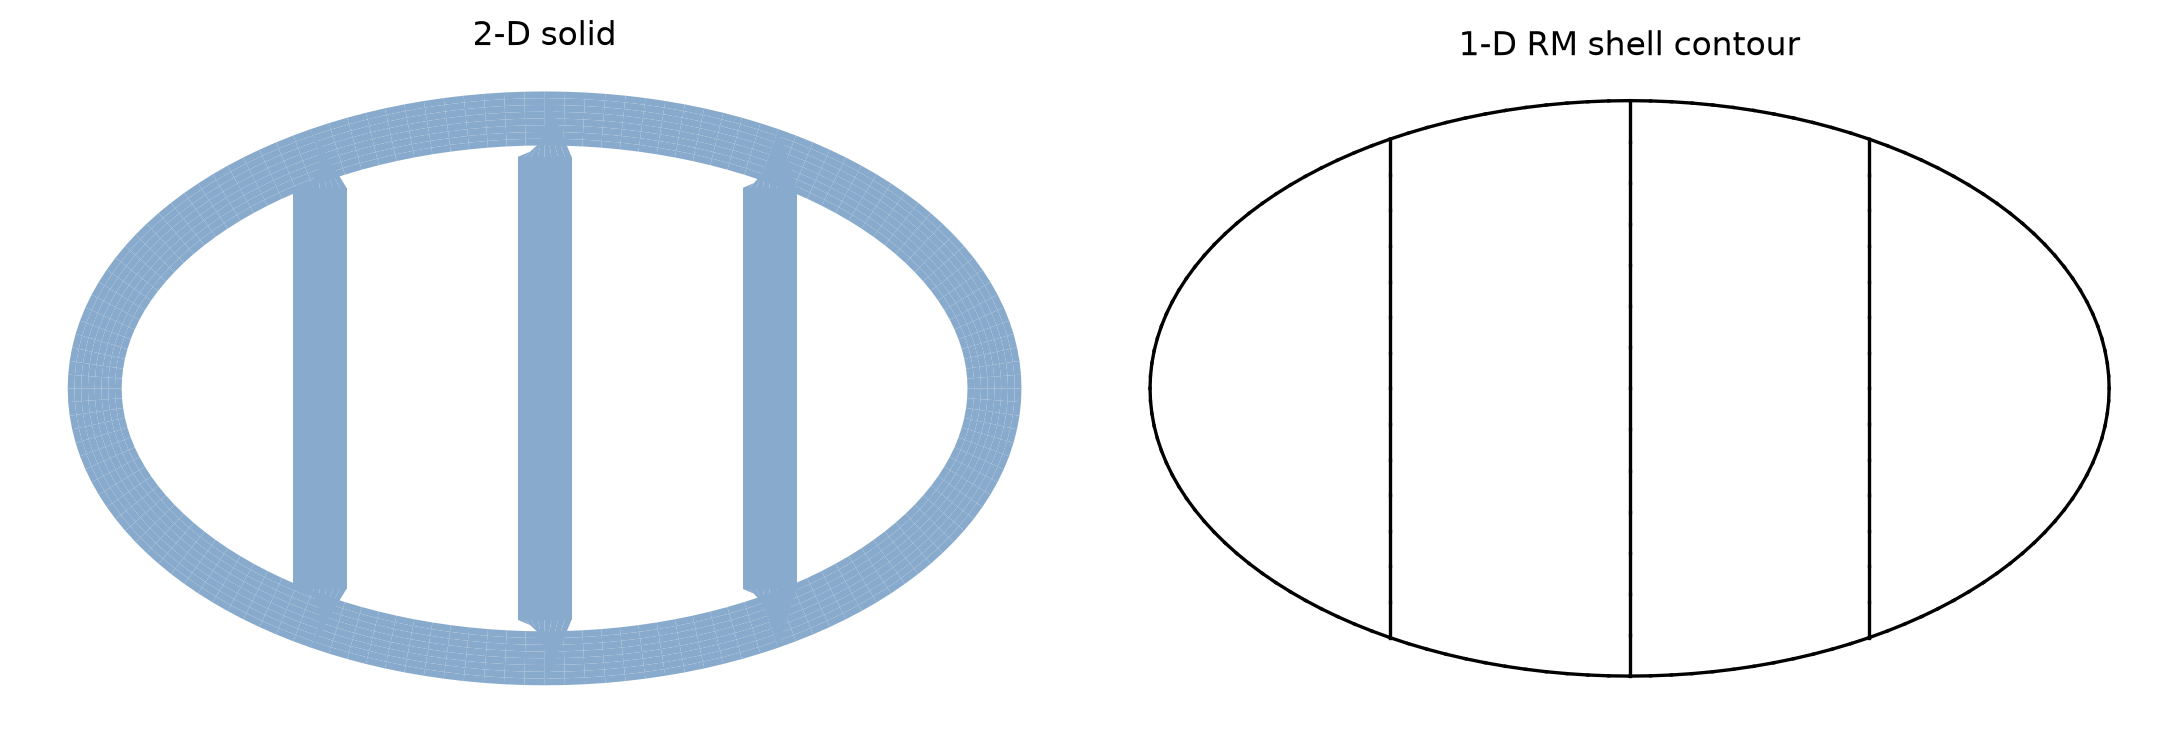
\includegraphics[width=0.72\textwidth]{figures/ell4cell_mesh.png}
\caption{Elliptic four-cell tube: 2-D solid mesh (filled by material) with the 1-D RM
shell mid-surface contour overlaid as the dotted centre reference.}\label{fig:ell4}
\end{figure}

\begin{table}[htpb]
\centering
\small
\caption{Elliptic four-cell tube (isotropic): RM 6-DOF shell vs.\ the 2-D solid, thin ($t/a=0.02$) and thick ($t/a=0.12$) wall ($\times10^{9}$).}
\label{tab:elliso}
\setlength{\tabcolsep}{4.5pt}
\begin{tabular}{l|rrr|rrr}
\hline
 & \multicolumn{3}{c|}{thin} & \multicolumn{3}{c}{thick} \\
$C^{b}_{ij}$ & solid & shell & \%err & solid & shell & \%err \\
\hline
$C^{b}_{11}$ & $11.42$ & $11.74$ & $+2.8$ & $68.87$ & $70.42$ & $+2.3$ \\
$C^{b}_{22}$ & $1.709$ & $1.708$ & $-0.1$ & $10.35$ & $10.29$ & $-0.5$ \\
$C^{b}_{33}$ & $2.456$ & $2.503$ & $+1.9$ & $15.05$ & $15.11$ & $+0.4$ \\
$C^{b}_{44}$ & $1.598$ & $1.601$ & $+0.2$ & $9.699$ & $9.703$ & $+0.0$ \\
$C^{b}_{55}$ & $1.82$ & $1.907$ & $+4.8$ & $11.1$ & $11.48$ & $+3.4$ \\
$C^{b}_{66}$ & $3.814$ & $3.864$ & $+1.3$ & $23.06$ & $23.23$ & $+0.7$ \\
\hline
\end{tabular}
\end{table}
\begin{table}[htpb]
\centering
\small
\caption{Elliptic four-cell tube ($[-45^\circ]$): RM 6-DOF shell vs.\ the 2-D solid, thin ($t/a=0.02$) and thick ($t/a=0.12$) wall (diagonal constants; the sign-odd couplings depend on the web through-thickness convention and are omitted) ($\times10^{9}$).}
\label{tab:ellm45}
\setlength{\tabcolsep}{4.5pt}
\begin{tabular}{l|rrr|rrr}
\hline
 & \multicolumn{3}{c|}{thin} & \multicolumn{3}{c}{thick} \\
$C^{b}_{ij}$ & solid & shell & \%err & solid & shell & \%err \\
\hline
$C^{b}_{11}$ & $1.994$ & $2.048$ & $+2.7$ & $12.02$ & $12.28$ & $+2.2$ \\
$C^{b}_{22}$ & $0.4207$ & $0.3102$ & $-26.3$ & $3.111$ & $3.092$ & $-0.6$ \\
$C^{b}_{33}$ & $0.6476$ & $0.6642$ & $+2.6$ & $3.979$ & $4.03$ & $+1.3$ \\
$C^{b}_{44}$ & $0.4384$ & $0.4395$ & $+0.3$ & $2.679$ & $2.679$ & $-0.0$ \\
$C^{b}_{55}$ & $0.3118$ & $0.3165$ & $+1.5$ & $1.947$ & $1.996$ & $+2.5$ \\
$C^{b}_{66}$ & $0.6613$ & $0.6695$ & $+1.2$ & $4.001$ & $4.027$ & $+0.6$ \\
\hline
\end{tabular}
\end{table}

%----------------------------------------------------------------------------------
\subsection{Example 3: IEA-22 blade cross-section at $r/R=0.2$}\label{sec:res_iea}
The IEA-22 station at $r/R=0.2$ is a three-web box: carbon spar caps, foam-core sandwich
panels, and glass at the leading and trailing edges, drawn directly from the windIO
description (Section~\ref{sec:workflow}). The six constituent materials and the six wall
laminates they form at this station are listed in Tables~\ref{tab:iea_mat}
and~\ref{tab:iea_layup}. The 2-D solid reference is the PreVABS
cross-sectional mesh, homogenized by the 2-D-solid MSG solver; Figure~\ref{fig:iea_mesh}
shows both meshes. Table~\ref{tab:iea020} gives the term-by-term comparison with the OML
laminate reference: extension and both bendings within $2.2\%$, torsion within $2.8\%$,
chordwise shear within $2\%$, and flapwise shear within $5.6\%$. The four significant couplings---the extension--bending pair $C^{b}_{15},C^{b}_{16}$, the
shear--torsion $C^{b}_{34}$, and the bending--bending $C^{b}_{56}$---are reproduced within
$5\%$ (couplings more than three orders of magnitude below the leading stiffness are
omitted from the table).
Figure~\ref{fig:conv_iea} shows the mesh-convergence of the shell contour: extension,
torsion, and both bendings are settled to a fraction of a percent from the coarsest
contour ($132$ nodes), and the flapwise shear varies within a $\pm0.8\%$ band---the
reported differences are the RM model error, not discretization.

\begin{figure}[htbp]\centering
\begin{minipage}{0.49\textwidth}\centering
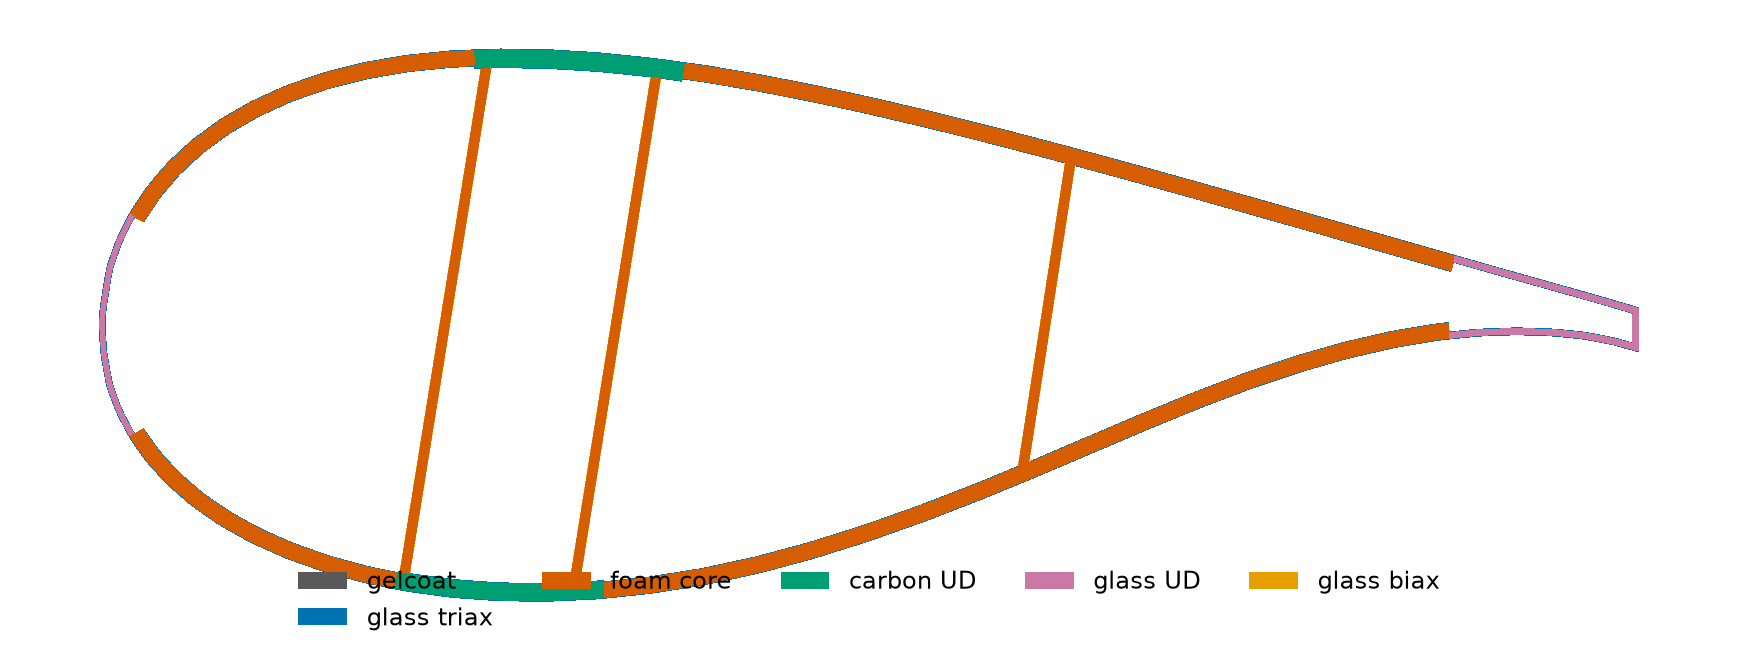
\includegraphics[width=\linewidth]{figures/iea_r020_solid_prevabs.png}\\[1pt]{\small (a) 2-D solid (PreVABS)}
\end{minipage}\hfill
\begin{minipage}{0.49\textwidth}\centering
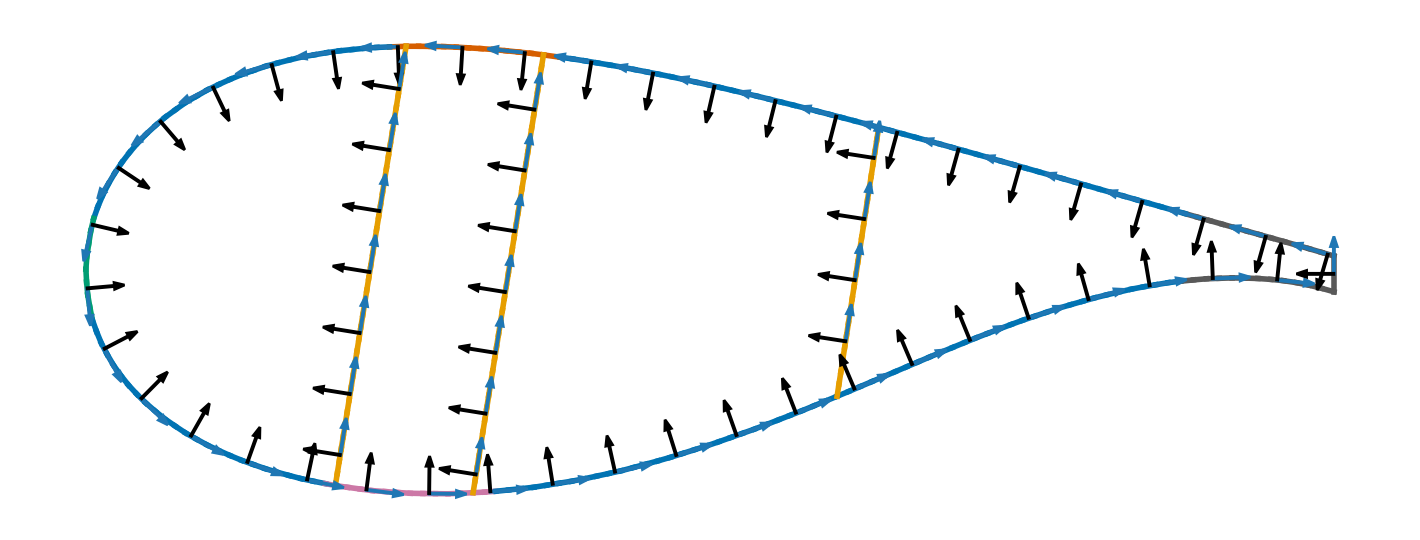
\includegraphics[width=\linewidth]{figures/iea_r020_shell.png}\\[1pt]{\small (b) 1-D RM shell}
\end{minipage}
\caption{IEA-22 cross-section at $r/R=0.2$: 2-D solid PreVABS mesh coloured by material
(left) and 1-D RM shell contour with the material frame (right).}\label{fig:iea_mesh}
\end{figure}

\begin{table}[htpb]
\centering
\caption{Constituent material properties of the IEA-22-280 blade laminates ($E$, $G$ in GPa; $\rho$ in kg/m$^3$).}
\label{tab:iea_mat}
\setlength{\tabcolsep}{5pt}
\resizebox{\textwidth}{!}{%
\begin{tabular}{lcccccccccc}
\hline
Material & $E_1$ & $E_2$ & $E_3$ & $G_{12}$ & $G_{13}$ & $G_{23}$ & $\nu_{12}$ & $\nu_{13}$ & $\nu_{23}$ & $\rho$ \\
\hline
Gelcoat        & 3.44 & 3.44 & 3.44 & 1.323 & 1.323 & 1.323 & 0.3 & 0.3 & 0.3 & 1235 \\
Glass triax    & 28.2 & 16.2 & 15.8 & 8.248 & 3.491 & 3.491 & 0.498 & 0.181 & 0.275 & 1940 \\
Glass uniax    & 43.7 & 16.5 & 15.4 & 3.265 & 3.495 & 3.48 & 0.262 & 0.264 & 0.35 & 1940 \\
Foam (MD)      & 0.142 & 0.142 & 0.142 & 0.054 & 0.054 & 0.054 & 0.319 & 0.319 & 0.319 & 130 \\
Carbon uniax   & 140 & 9.1 & 9.1 & 4.131 & 4.131 & 2.689 & 0.313 & 0.313 & 0.471 & 1600 \\
Glass biax     & 11 & 11 & 16 & 13.23 & 3.487 & 3.487 & 0.688 & 0.117 & 0.117 & 1940 \\
\hline
\end{tabular}%
}
\end{table}
\begin{table}[htpb]
\centering
\caption{Wall laminates (layups) of the $r/R=0.2$ section, grouped by structural region and listed from the outer mould line inward. Each row is one stack of identical plies; the layer thickness is the ply thickness times the number of plies.}
\label{tab:iea_layup}
\resizebox{\textwidth}{!}{%
\begin{tabular}{llclccc}
\hline
Name & Region & Layer & Material & Ply thickness (m) & Orientation ($^\circ$) & Number of plies \\
\hline
\multirow{4}{*}{layup\_0} & \multirow{4}{*}{Glass-uniax skin} & 1 & Gelcoat & 0.0005 & 0 & 1 \\
 &  & 2 & Glass triax & 0.003003 & 0 & 1 \\
 &  & 3 & Glass uniax & 0.02609 & 0 & 1 \\
 &  & 4 & Glass triax & 0.003003 & 0 & 1 \\
\hline
\multirow{4}{*}{layup\_1} & \multirow{4}{*}{Foam-cored panel} & 1 & Gelcoat & 0.0005 & 0 & 1 \\
 &  & 2 & Glass triax & 0.003003 & 0 & 1 \\
 &  & 3 & Foam (MD) & 0.07061 & 0 & 1 \\
 &  & 4 & Glass triax & 0.003003 & 0 & 1 \\
\hline
\multirow{4}{*}{layup\_2} & \multirow{4}{*}{Carbon spar cap} & 1 & Gelcoat & 0.0005 & 0 & 1 \\
 &  & 2 & Glass triax & 0.003003 & 0 & 1 \\
 &  & 3 & Carbon uniax & 0.08106 & 0 & 1 \\
 &  & 4 & Glass triax & 0.003003 & 0 & 1 \\
\hline
\multirow{4}{*}{layup\_3} & \multirow{4}{*}{Glass-uniax skin} & 1 & Gelcoat & 0.0005 & 0 & 1 \\
 &  & 2 & Glass triax & 0.003003 & 0 & 1 \\
 &  & 3 & Glass uniax & 0.02158 & 0 & 1 \\
 &  & 4 & Glass triax & 0.003003 & 0 & 1 \\
\hline
\multirow{4}{*}{layup\_4} & \multirow{4}{*}{Carbon spar cap} & 1 & Gelcoat & 0.0005 & 0 & 1 \\
 &  & 2 & Glass triax & 0.003003 & 0 & 1 \\
 &  & 3 & Carbon uniax & 0.07707 & 0 & 1 \\
 &  & 4 & Glass triax & 0.003003 & 0 & 1 \\
\hline
\multirow{3}{*}{layup\_5} & \multirow{3}{*}{Shear web} & 1 & Glass biax & 0.002 & 0 & 1 \\
 &  & 2 & Foam (MD) & 0.042 & 0 & 1 \\
 &  & 3 & Glass biax & 0.002 & 0 & 1 \\
\hline
\end{tabular}%
}
\end{table}
\begin{table}[htpb]
\centering
\small
\caption{IEA-22 blade cross-section at $r/R=0.2$ (OML reference): RM 6-DOF shell vs.\ the 2-D solid ($\times10^{9}$).}
\label{tab:iea020}
\setlength{\tabcolsep}{4.5pt}
\begin{tabular}{l|rrr}
\hline
 & \multicolumn{3}{c}{} \\
$C^{b}_{ij}$ & solid & shell & \%err \\
\hline
$C^{b}_{11}$ & $28.07$ & $27.96$ & $-0.4$ \\
$C^{b}_{15}$ & $1.685$ & $1.624$ & $-3.6$ \\
$C^{b}_{16}$ & $-70.38$ & $-71.46$ & $+1.5$ \\
$C^{b}_{22}$ & $0.7341$ & $0.7198$ & $-1.9$ \\
$C^{b}_{33}$ & $0.431$ & $0.407$ & $-5.6$ \\
$C^{b}_{34}$ & $0.8861$ & $0.8417$ & $-5.0$ \\
$C^{b}_{44}$ & $4.195$ & $4.079$ & $-2.8$ \\
$C^{b}_{55}$ & $35.19$ & $35.49$ & $+0.8$ \\
$C^{b}_{56}$ & $-9.716$ & $-9.645$ & $-0.7$ \\
$C^{b}_{66}$ & $246.5$ & $251.9$ & $+2.2$ \\
\hline
\end{tabular}
\end{table}

The five-parameter drilling-eliminated element was also run on the same ring
($1{,}560$ field DOF against $1{,}872$ plus $315$ element multipliers on the
$312$-node reference contour): it reproduces the classical constants
identically and lands \emph{closer} to the solid on the flapwise shear and torsion
($C^{b}_{33}$ $-3.7\%$ vs.\ $-5.6\%$, $C^{b}_{44}$ $-2.1\%$ vs.\ $-2.8\%$ at $r/R=0.2$).
This is not superior accuracy but error cancellation: the elimination systematically
\emph{stiffens} the shear and torsion channels carried by the webs---pure error of
$+8.3\%$ on the two-cell tube where the wall model itself is nearly exact---and on the
blade this spurious stiffening partially offsets the RM wall model's genuine shear
undershoot. The constrained six-parameter element is the formulation-consistent one; its
residual is the model error itself, not two errors in fortuitous opposition.

\begin{figure}[htbp]\centering
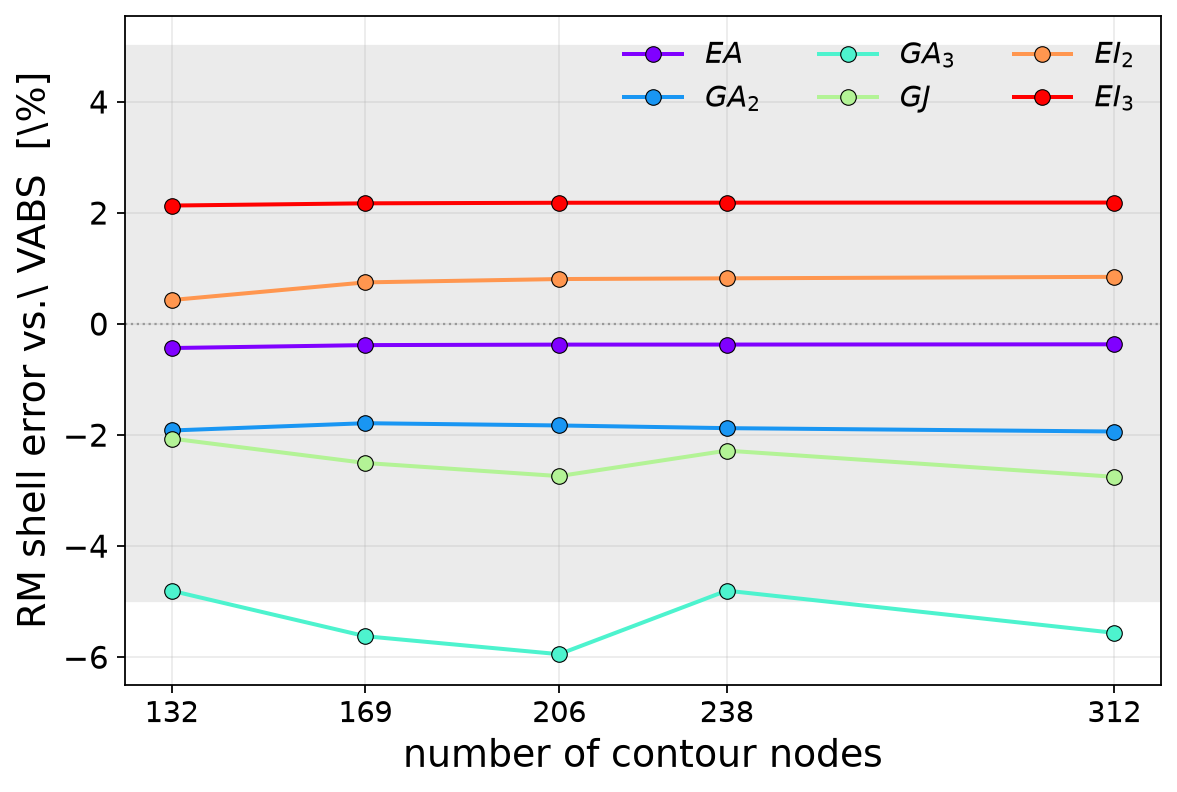
\includegraphics[width=0.62\textwidth]{figures/conv_iea_r020.png}
\caption{IEA-22 $r/R=0.2$: RM 6-DOF diagonal \% error vs.\ shell-contour node count
(OML reference; the 2-D solid reference is fixed).}\label{fig:conv_iea}
\end{figure}

%----------------------------------------------------------------------------------
\subsection{Example 4: the full IEA-22 blade}\label{sec:res_blade}
Homogenizing at the \emph{actual} windIO airfoil-definition stations assembles the blade's
complete one-dimensional beam model on the real section geometries, with no interpolated
stations. The IEA-22 windIO description places its airfoils at the \texttt{spanwise\_position}
entries FFA-W3-330blend, -301, -270blend, -241 and -211 ($r=0.247,0.399,0.534,0.739$ and
$0.980$); together with the $r=0.2$ root section of Examples~3 and~5 these are the six stations
used here. This repeats the full-blade verification of the Kirchhoff--Love companion study
\cite{bagla2024asc,camarena2025} with the single RM 6-DOF element, now against a full VABS
analysis of the 2-D solid at each station. Figure~\ref{fig:span_loft} lofts representative
cross-sections along the beam reference axis to show the taper.

Table~\ref{tab:fullblade_real} and Figure~\ref{fig:span} give the RM shell against the VABS
solid. The full $6\times6$ agrees to a Frobenius error of $1.5$--$2.4\%$ at \emph{every}
station; extension and both bendings track VABS within $1.5\%$, $1.4\%$ and---bar the thin
$r=0.98$ tip ($+6.2\%$ on $EI_3$)---about $2\%$, and the chordwise shear $GA_2$ within $3.2\%$.
The flapwise transverse shear $GA_3$ ($-5\%$ to $-11\%$) and the torsion $GJ$ ($-3\%$ to $-9\%$)
drift outboard: the transverse-shear-flexible sandwich walls thin faster than the section
contracts, so the single-director wall progressively under-resolves the through-thickness shear.
Each station homogenizes in about one second.

\begin{figure}[htbp]\centering
\begin{minipage}[c]{0.86\textwidth}\centering
\includegraphics[width=\textwidth]{figures/iea_span_loft_noleg.png}
\end{minipage}\hfill
\begin{minipage}[c]{0.12\textwidth}\centering
\includegraphics[width=\textwidth]{figures/iea_span_legend.png}
\end{minipage}
\caption{Representative IEA-22 cross-sections lofted along the beam reference axis (dotted),
coloured by wall region, illustrating the blade taper; the $6\times6$ comparison
(Table~\ref{tab:fullblade_real}) is taken at the windIO airfoil stations.}\label{fig:span_loft}
\end{figure}

\begin{table}[t]\centering\small
\caption{Full IEA-22 blade at the \emph{actual} windIO airfoil stations: RM 6-DOF shell cross-section vs.\ the VABS 2-D solid ($.\mathrm{K}$) --- diagonal \%\,error and full $6\times6$ Frobenius error. Stations are the windIO \texttt{spanwise\_position} entries (airfoil in parentheses); $r=0.2$ is the root example section.}\label{tab:fullblade_real}
\begin{tabular}{llrrrrrrr}
\toprule
$r$ & airfoil & $EA$ & $GA_2$ & $GA_3$ & $GJ$ & $EI_2$ & $EI_3$ & Frob.\\
\midrule
$0.200$ & FFA-root & $-0.4$ & $-1.9$ & $-5.5$ & $-2.7$ & $+0.8$ & $+2.2$ & $2.1\%$\\
$0.247$ & FFA-330blend & $+0.2$ & $-0.5$ & $-5.2$ & $-3.0$ & $+0.9$ & $+2.1$ & $2.0\%$\\
$0.399$ & FFA-301 & $+1.4$ & $+2.0$ & $-7.8$ & $-4.2$ & $+1.4$ & $+2.0$ & $1.9\%$\\
$0.534$ & FFA-270blend & $+1.5$ & $+2.8$ & $-10.0$ & $-5.8$ & $+1.4$ & $+1.8$ & $1.7\%$\\
$0.739$ & FFA-241 & $+1.4$ & $+3.2$ & $-11.0$ & $-8.5$ & $+1.2$ & $+1.8$ & $1.5\%$\\
$0.980$ & FFA-211 & $+1.5$ & $+0.2$ & $-9.2$ & $-9.0$ & $+0.6$ & $+6.2$ & $2.4\%$\\
\bottomrule
\end{tabular}
\end{table}

\begin{figure}[htbp]\centering
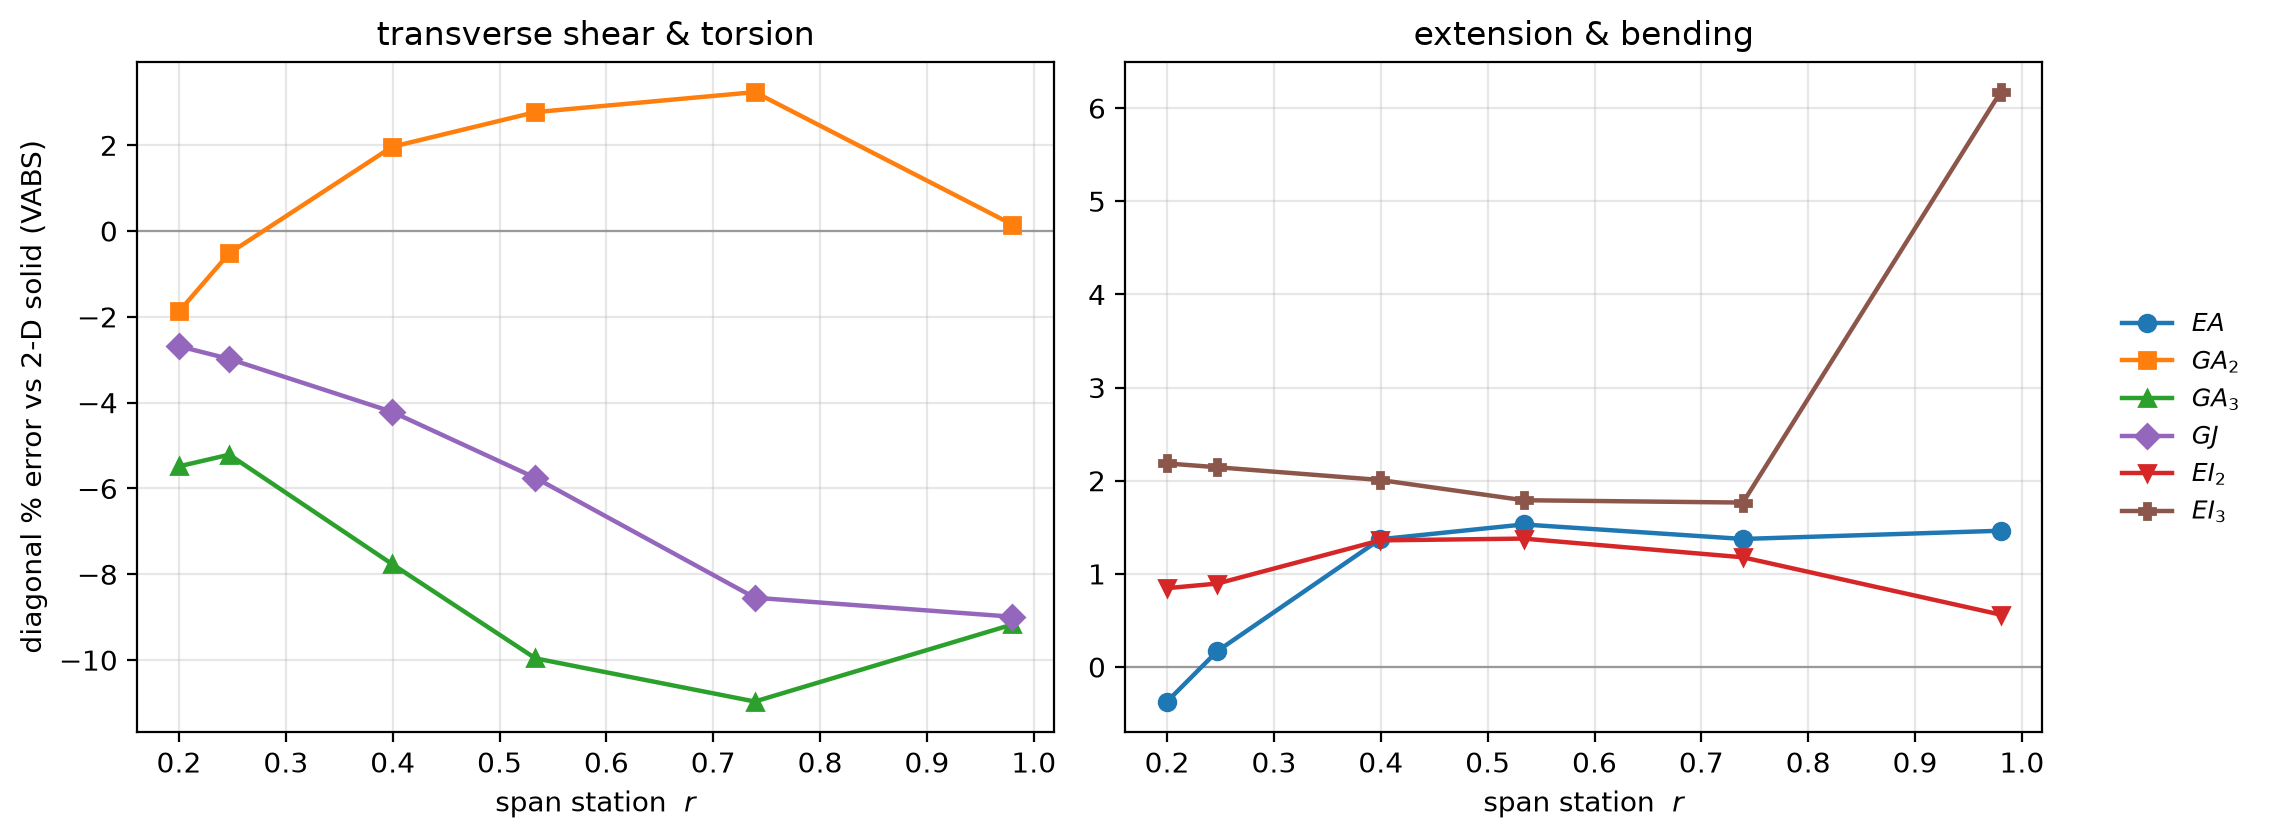
\includegraphics[width=\textwidth]{figures/full_blade_rm_span_real.png}
\caption{Full IEA-22 blade at the windIO airfoil stations: RM 6-DOF cross-section diagonal
\% error vs.\ the VABS 2-D solid across the span (left: transverse shear and torsion; right:
extension and bending), OML laminate reference.}\label{fig:span}
\end{figure}

%----------------------------------------------------------------------------------
\subsection{Computational cost}\label{sec:res_cost}
Table~\ref{tab:timing4} tabulates the wall-clock solver cost of the three homogenizers
on all four examples: the present 1-D RM shell ring, the OpenSG-JAX 2-D solid, and the
OpenSG-FEniCS 2-D solid on the same mesh. The two independent 2-D solids agree on the
section constants---a cross-check of the reference itself. At these section sizes the
solve times are of the same order for all three methods (the compiled JAX solid is even
marginally faster on the blade sections); the structural advantages of the 1-D contour
lie elsewhere: it assembles $2$--$4\times$ fewer unknowns, it requires no
through-thickness meshing of the wall---the entire ply stack enters through the
$8\times8$ wall law, so the cost is independent of the ply count, whereas the 2-D solid
mesh grows with every ply resolved---and the complete eight-station blade model is
assembled in a few seconds end to end.

\begin{table}[t]\centering\small
\caption{Wall-clock solver cost of the three homogenizers on the four examples: the RM 6-DOF shell ring (1-D contour), the OpenSG-JAX 2-D solid, and the OpenSG-FEniCS 2-D solid (same mesh). JAX time is the compiled-kernel solve; its one-off JIT compilation and all mesh generation are excluded. DOF counts are the displacement/rotation unknowns (the RM ring additionally carries one Lagrange multiplier per element); the $r/R=0.2$ row times the medium ($206$-node) contour of the convergence study, not the $312$-node reference contour. The blade row sums all eight stations.}\label{tab:timing4}
\setlength{\tabcolsep}{5pt}
\begin{tabular}{l|rr|rr|rr}
\toprule
& \multicolumn{2}{c|}{RM shell (1-D)} & \multicolumn{2}{c|}{JAX 2-D solid} & \multicolumn{2}{c}{FEniCS 2-D solid}\\
example & DOF & $t$ (s) & DOF & $t$ (s) & DOF & $t$ (s)\\
\midrule
two-cell tube & 1434 & $0.28$ & 3585 & $1.45$ & 3585 & $0.49$\\
elliptic four-cell & 1098 & $0.66$ & 4941 & $2.13$ & 4941 & $0.53$\\
IEA-22 $r/R=0.2$ & 1236 & $0.73$ & 2559 & $0.59$ & 2559 & $1.28$\\
full IEA-22 blade (8 stations) & --- & $5.28$ & --- & $4.33$ & --- & $10.79$\\
\bottomrule
\end{tabular}
\end{table}

%----------------------------------------------------------------------------------
\subsection{Example 5: local field recovery by dehomogenization}\label{sec:res_dehom}
Cross-sectional analysis is invertible: the same warping fields that condense the
three-dimensional problem into the beam $6\times6$ can \emph{recover} the pointwise 3-D
stress and displacement from the beam internal loads---the \emph{dehomogenization} step,
which is what makes a beam model usable for strength. We demonstrate it on the IEA-22 root
section at $r=0.2$ (the same blade as Examples~3 and~3.1; a $7.2$~m chord with three shear
webs and carbon spar caps whose wall is $\sim\!88$~mm thick), and compare the RM shell
two-step recovery against a full VABS analysis of the \emph{same} PreVABS $2$-D solid mesh.
The section, its material regions and the two sampling paths---a through-thickness column at
the LP spar-cap centre and a circumferential path along the LP (suction) surface from the
leading to the trailing edge---are shown in Figure~\ref{fig:r020_section}; both paths are
taken directly on the solid outer mould line.

\begin{figure}[htbp]\centering

\includegraphics[width=\textwidth]{figures/r020_section_paths.png}
\caption{IEA $r=0.2$ root section (PreVABS $2$-D solid, coloured by material) with the two
dehomogenization paths: the LP-surface circumferential path (blue, LE$\to$TE) and the
spar-cap through-thickness column (red), both on the solid OML.}\label{fig:r020_section}
\end{figure}

Homogenization comes first: Table~\ref{tab:r020_homo} lists every nonzero $C_{ij}$ of the RM
shell---the same $C^0$ drilling-constrained, MITC-$\gamma_{23}$ ring used everywhere else in
this paper, at the OML reference---against the VABS $.\mathrm{K}$ of the solid. The full
$6\times6$ agrees to a Frobenius error of $2.1\%$, every diagonal within a few percent, so the
RM $6\times6$ that the dehomogenization inverts is a faithful model of the solid.

\begin{table}[htpb]\centering\small
\caption{IEA r$=0.2$ root Timoshenko $6\times6$: every nonzero $C_{ij}$ of the RM shell (the $C^0$ MITC-$\gamma_{23}$ ring, OML) vs.\ the VABS $.\mathrm{K}$ (2-D solid). VABS order $[1\!=\!\mathrm{ext},2,3\!=\!\mathrm{shear},4\!=\!\mathrm{twist},5,6\!=\!\mathrm{bend}]$.}\label{tab:r020_homo}
\begin{tabular}{lrrr}
\toprule
$C_{ij}$ & VABS $.\mathrm{K}$ & RM shell & \%\,err \\
\midrule
$C_{11}\,(EA)$ & $2.807e+10$ & $2.796e+10$ & $-0.4$ \\
$C_{15}$ & $1.685e+09$ & $1.624e+09$ & $-3.6$ \\
$C_{16}$ & $-7.038e+10$ & $-7.146e+10$ & $+1.5$ \\
$C_{22}\,(GA_2)$ & $7.336e+08$ & $7.198e+08$ & $-1.9$ \\
$C_{33}\,(GA_3)$ & $4.306e+08$ & $4.070e+08$ & $-5.5$ \\
$C_{34}$ & $8.856e+08$ & $8.417e+08$ & $-5.0$ \\
$C_{44}\,(GJ)$ & $4.192e+09$ & $4.079e+09$ & $-2.7$ \\
$C_{55}\,(EI_2)$ & $3.519e+10$ & $3.549e+10$ & $+0.8$ \\
$C_{56}$ & $-9.716e+09$ & $-9.645e+09$ & $-0.7$ \\
$C_{66}\,(EI_3)$ & $2.465e+11$ & $2.519e+11$ & $+2.2$ \\
\midrule
\multicolumn{4}{l}{\small full-$6\times6$ Frobenius error $=2.1\%$} \\
\bottomrule
\end{tabular}
\end{table}

Given a beam force $F$, the recovery is two steps
(Section~\ref{sec:wall}). Crucially, step~1 is driven by the \emph{same} Reissner--Mindlin
ring used for the homogenization---the $C^0$ drilling-constrained element with the
MITC-tied $\gamma_{23}$, not a Kirchhoff--Love shell---so the recovered shell strains are
consistent with the $6\times6$ they invert: the beam strain
$\bar{\epsilon}=\mathbf{S}^{-1}F$ (with $\mathbf{S}$ the RM Timoshenko stiffness) drives the
RM warping $V_0,V_1$ through the element strain operator to the eight shell strains
$[\epsilon_{11},\epsilon_{22},2\epsilon_{12},\kappa_{11},\kappa_{22},2\kappa_{12},
2\gamma_{13},2\gamma_{23}]$ along the contour. This recovery is the exact adjoint of the
RM assembly, so it is energy-consistent by construction. At each through-thickness depth the
same plate structure-gene that built the $8\times8$ then returns the local 3-D stress,
$\Sigma(\zeta_3)=C(\zeta_3)\,[\mathbf{B}(\zeta_3)V_0+G_e(\zeta_3)]\,\bar{\epsilon}$. We apply
the same beam load to the RM recovery and to the VABS solid recovery, and compare on the two
paths; Figures~\ref{fig:dehom_r020_circ} and~\ref{fig:dehom_r020_cap} show the result.

\begin{figure}[htbp]\centering

\includegraphics[width=\textwidth]{figures/dehom_r020_circumferential.png}
\caption{Circumferential path (LP suction surface, LE$\to$TE): RM shell two-step
dehomogenization vs.\ VABS $.\mathrm{SM}$. The dominant axial stress $\sigma_{11}$ (the
spanwise bending distribution, $-0.5$ to $+0.13$~MPa) overlaps VABS along the entire
surface; $\sigma_{22}$ tracks the web-junction steps. The transverse components (note the
axis scale, $\lesssim\!0.006$~MPa) are the plate plane-stress limit.}\label{fig:dehom_r020_circ}
\end{figure}

\begin{figure}[htbp]\centering
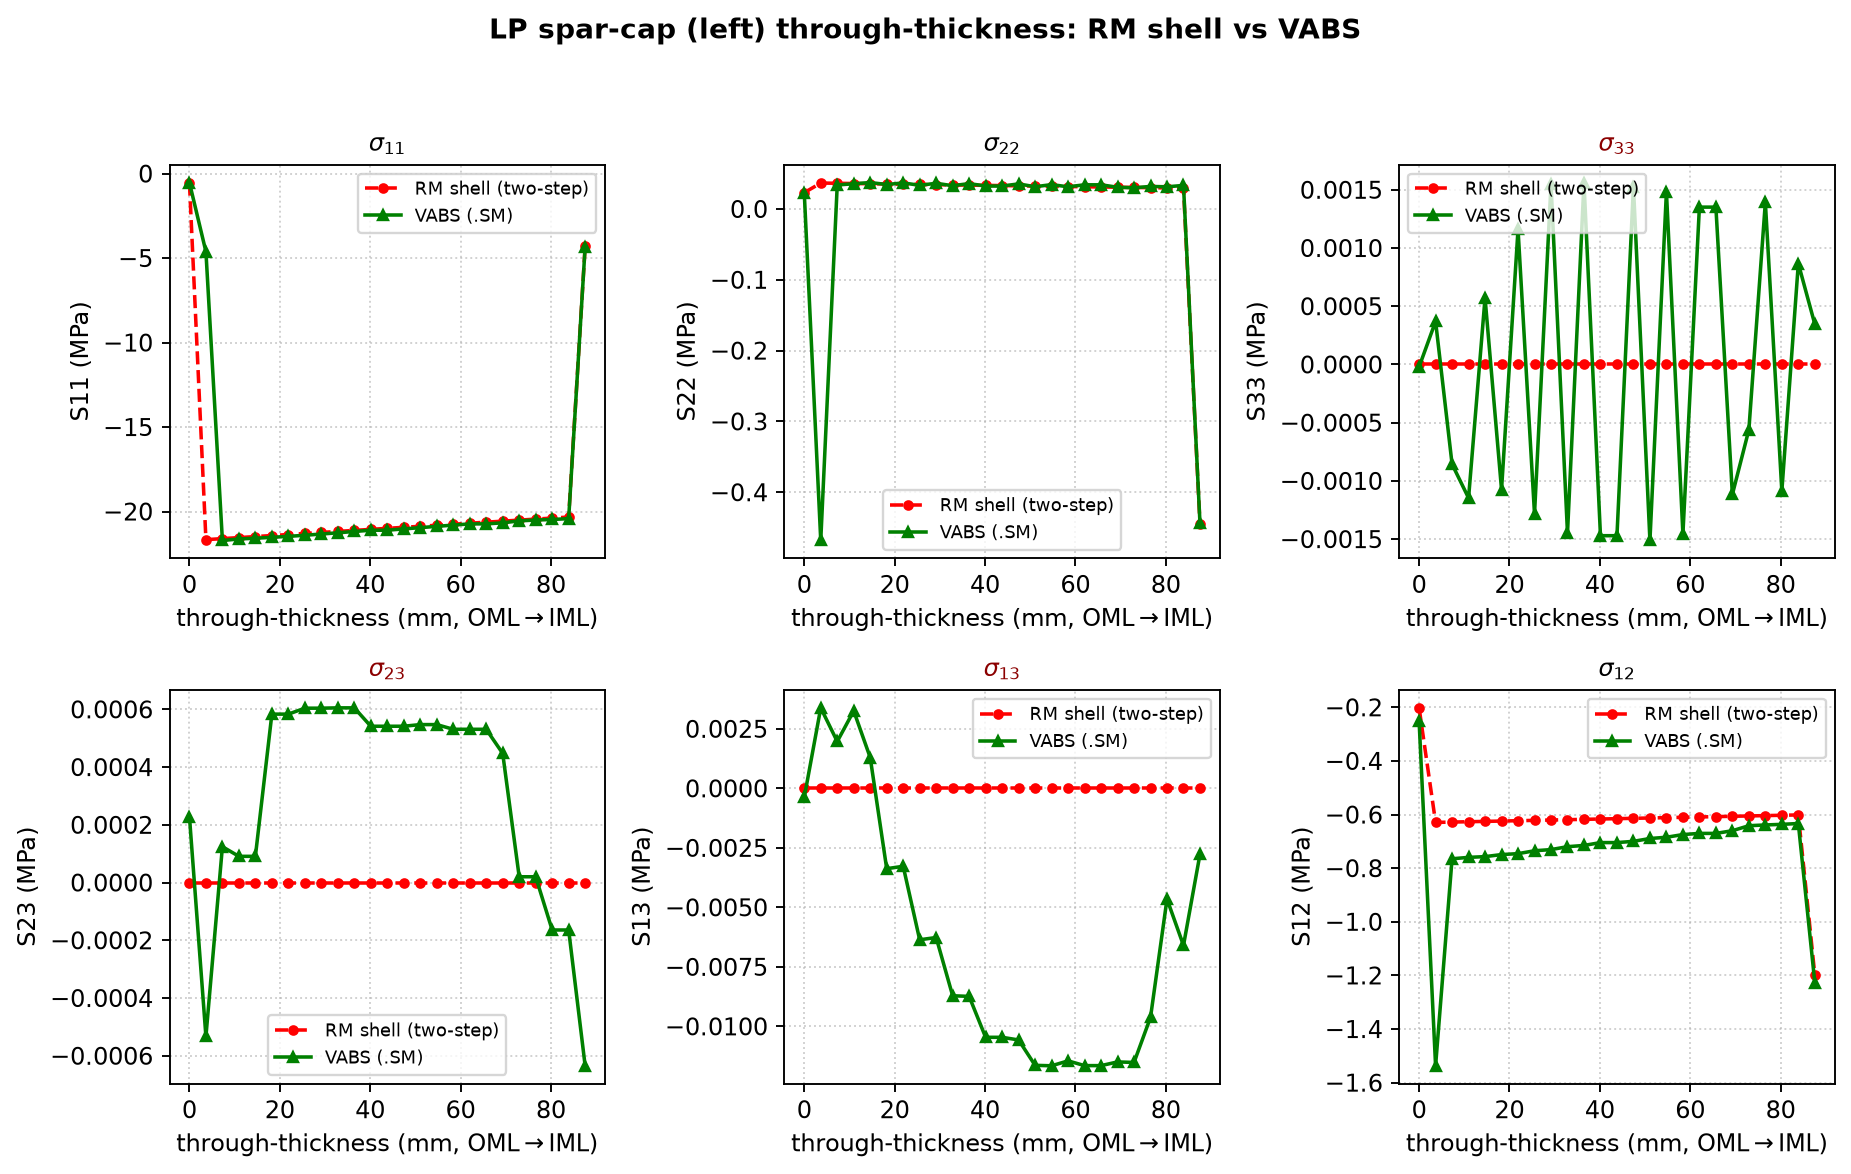
\includegraphics[width=\textwidth]{figures/dehom_r020_capleft.png}
\caption{LP spar-cap through-thickness (left of the cap, OML$\to$IML, $88$~mm): RM shell vs.\
VABS. The in-plane $\sigma_{11}$ overlaps VABS through the full carbon cap
($\approx\!-21$~MPa); the endpoint departures are the thin glass facesheets, where the stress
transitions over a few plies.}\label{fig:dehom_r020_cap}
\end{figure}

The agreement is field-wide, not only on the two paths. Figure~\ref{fig:r020_contour} contours
the in-plane stress over the whole section, VABS solid beside the RM shell recovery: the
strength-driving $\sigma_{11}$ (bending compression in the LP cap, tension in the HP cap) is
reproduced point-for-point, while $\sigma_{22}$ and $\sigma_{12}$ are one to two orders
smaller. The transverse-normal $\sigma_{33}$ and the transverse shears
$\sigma_{13},\sigma_{23}$ are three to four orders below the in-plane and are reported at the
plate plane-stress limit; a physical $\sigma_{13},\sigma_{23}$ (an equilibrium shear-flow
effect rather than a local constitutive one) is left to future work.

\begin{figure}[htbp]\centering

\includegraphics[width=\textwidth]{figures/r020_stress_contour_cmp.png}
\caption{In-plane stress over the section, VABS solid (left) vs.\ OpenSG RM shell
dehomogenization (right) for $\sigma_{11},\sigma_{22},\sigma_{12}$ (shared scale per row). The
strength-driving $\sigma_{11}$ matches; the smaller components differ mainly in the web shear
flow.}\label{fig:r020_contour}
\end{figure}

Dehomogenization also recovers the full local \emph{displacement} state. Along the LP
circumferential path the recovered warping $u_1,u_2,u_3$ tracks VABS
(Figure~\ref{fig:r020_disp_circ})---the axial warping $u_1$ within $\sim\!0.05$~mm over the
$8$~m surface and the in-plane $u_2,u_3$ essentially on top of the solid recovery. The
agreement is field-wide: Figure~\ref{fig:r020_disp_contour} contours all three warping
components over the whole section, VABS solid beside the RM shell recovery, and the patterns
coincide point-for-point; the total displacement magnitude $|u|=\sqrt{u_1^2+u_2^2+u_3^2}$
(Figure~\ref{fig:r020_mag}) is likewise reproduced across the cross-section.

\begin{figure}[htbp]\centering
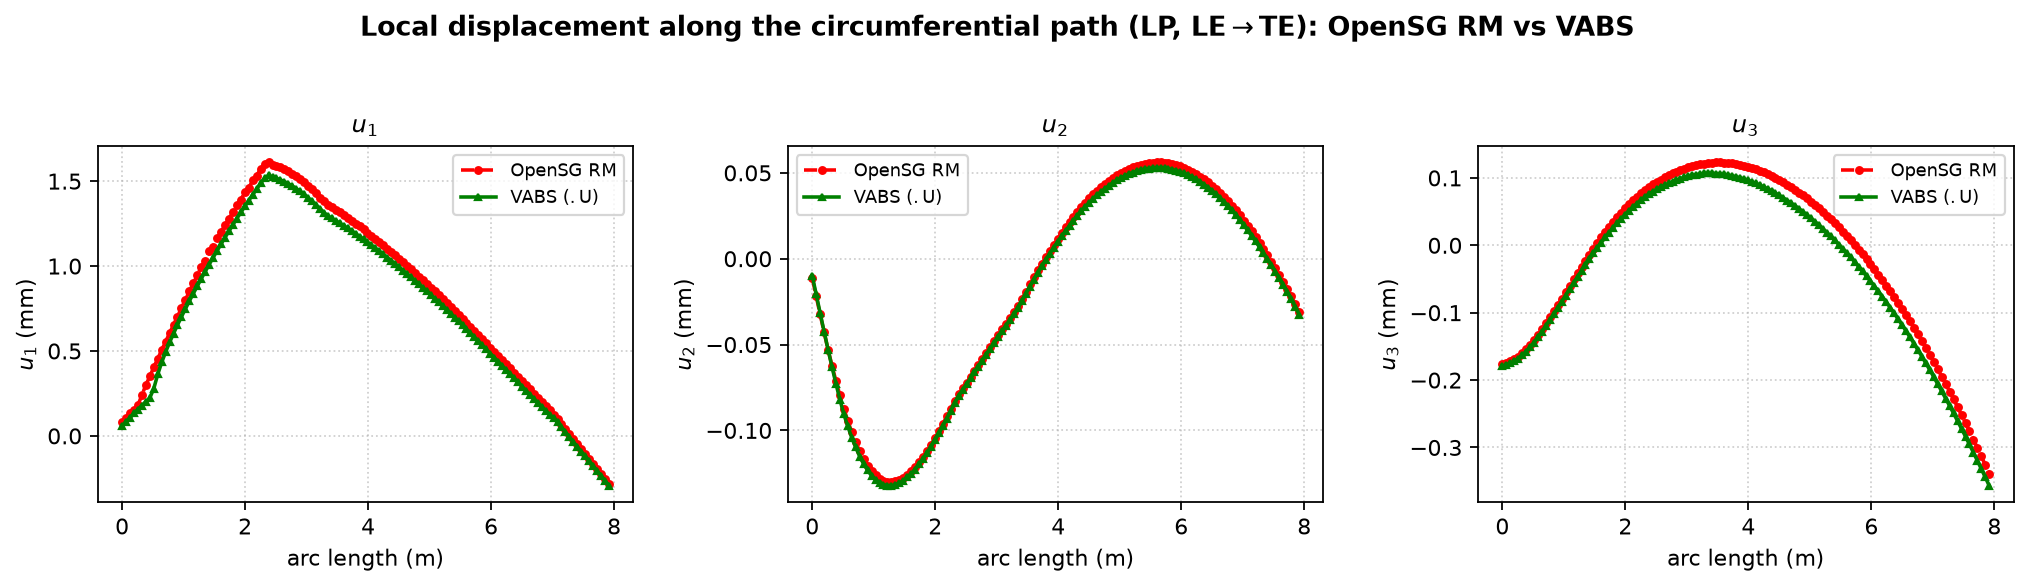
\includegraphics[width=\textwidth]{figures/r020_disp_circ.png}
\caption{Recovered warping displacement $u_1,u_2,u_3$ along the LP circumferential path
(LE$\to$TE): OpenSG RM shell dehomogenization vs.\ VABS $.\mathrm{U}$. All three components
overlap the solid recovery along the entire surface.}\label{fig:r020_disp_circ}
\end{figure}

\begin{figure}[htbp]\centering

\includegraphics[width=\textwidth]{figures/r020_disp_contour_cmp.png}
\caption{Local warping displacement $u_1,u_2,u_3$ over the section, VABS solid (left) vs.\
OpenSG RM shell dehomogenization (right), shared scale per row. The axial warping $u_1$ and the
in-plane $u_2,u_3$ are reproduced across the whole cross-section.}\label{fig:r020_disp_contour}
\end{figure}

\begin{figure}[htbp]\centering
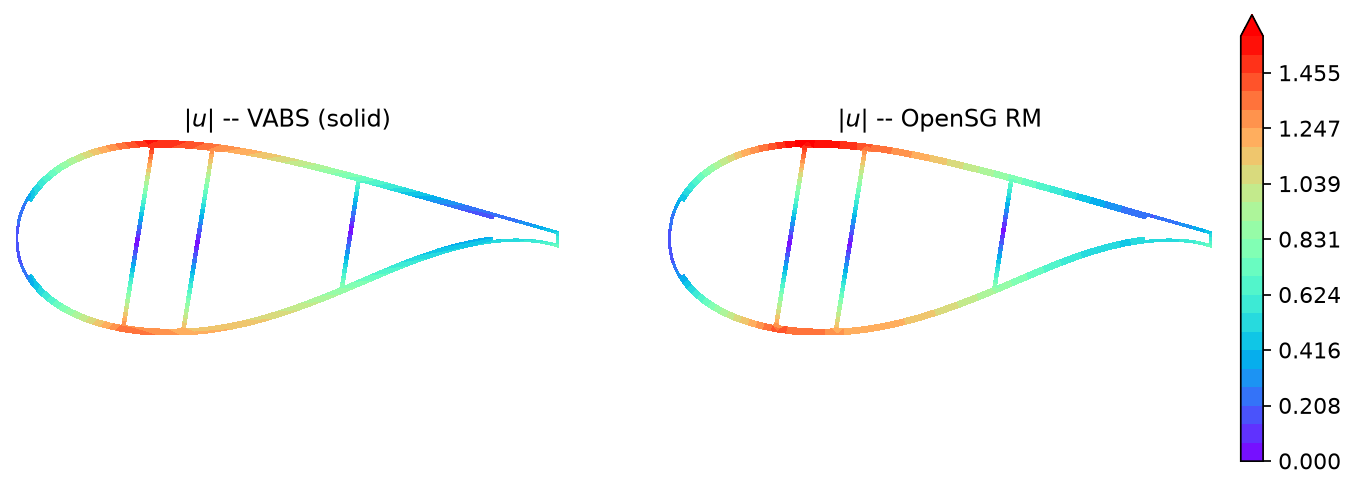
\includegraphics[width=\textwidth]{figures/r020_disp_mag.png}
\caption{Total local displacement magnitude $|u|=\sqrt{u_1^2+u_2^2+u_3^2}$ over the section:
VABS solid (left) vs.\ OpenSG RM shell dehomogenization (right). The combined warping field is
reproduced across the whole cross-section.}\label{fig:r020_mag}
\end{figure}

The recovery is not confined to the root. Applying each station's own VABS beam load, the RM
two-step dehomogenization reproduces the VABS local field along the whole blade at the windIO
airfoil stations of Example~4. Figure~\ref{fig:span_dehom} traces the in-plane stress and the
displacement at the section crown across the span: the axial $\sigma_{11}$ recovered by the
$1$-D RM solve lies on the VABS solid recovery at every station ($-2.05$ vs.\ $-2.07$~MPa at
$r=0.247$, $+0.15$ vs.\ $+0.15$~MPa at $r=0.98$), and the local displacement tracks within
$\sim\!5\%$ ($3.08$ vs.\ $2.98$~mm at $r=0.247$ down to $0.11$ vs.\ $0.11$~mm at the tip). A
single one-dimensional Reissner--Mindlin element thus recovers the pointwise three-dimensional
stress and displacement of the full composite blade section, everywhere along the span.

\begin{figure}[htbp]\centering
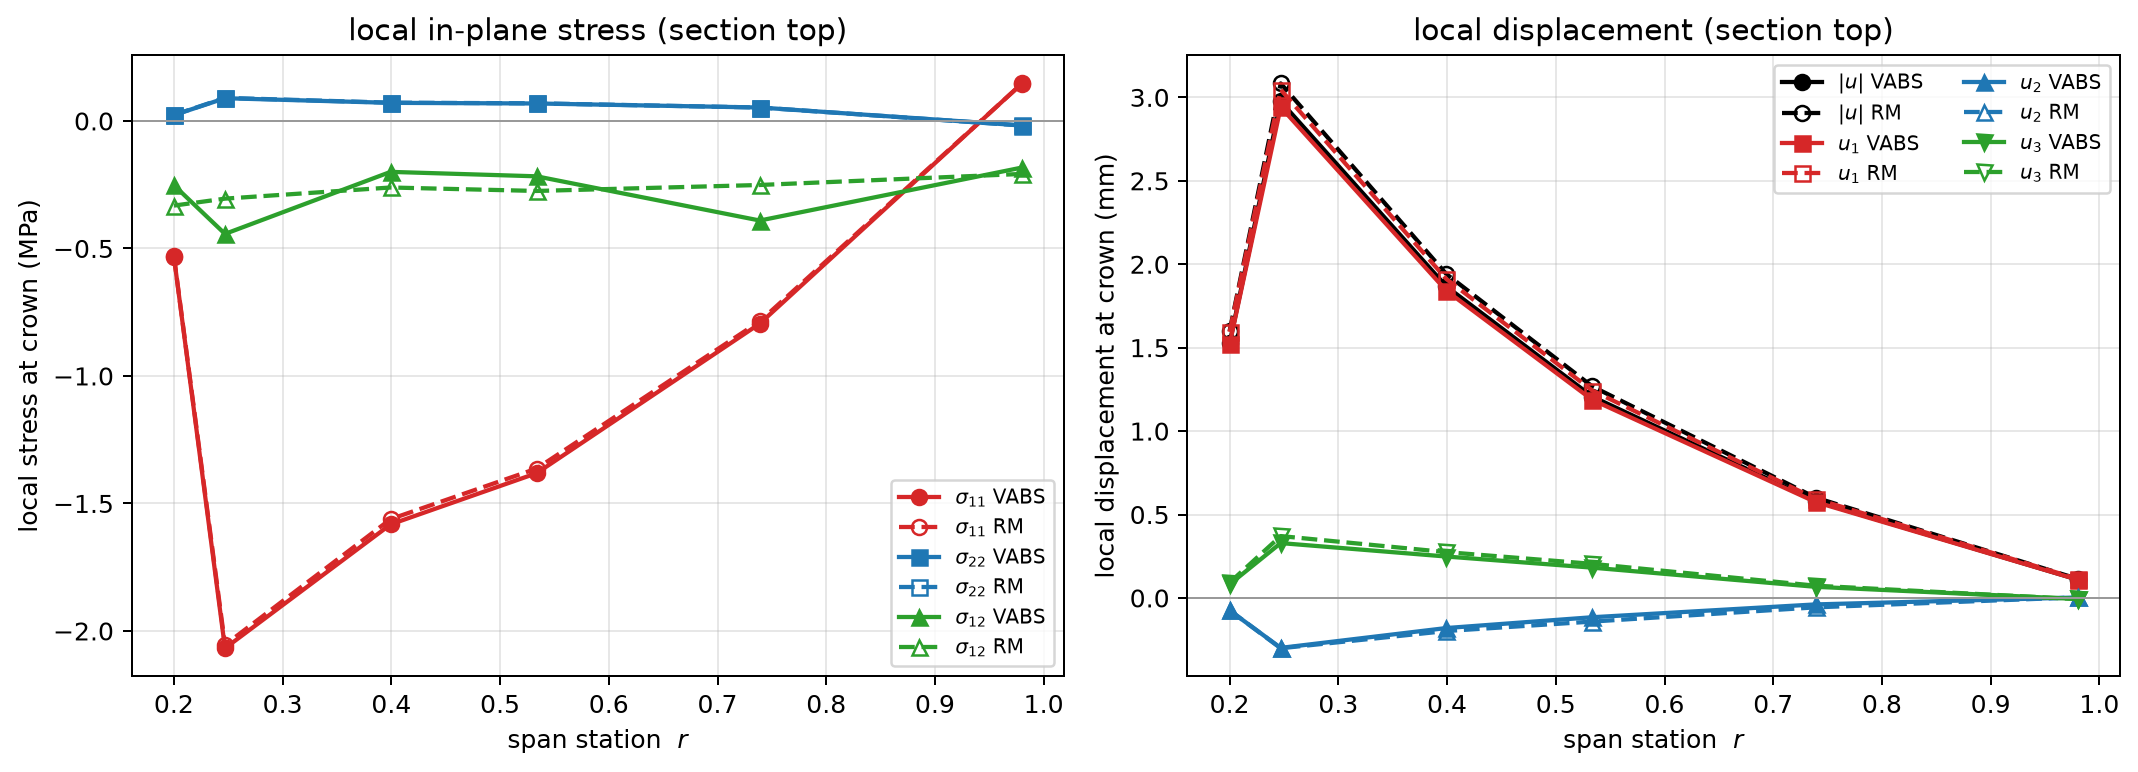
\includegraphics[width=\textwidth]{figures/span_dehom.png}
\caption{Spanwise dehomogenization at the windIO airfoil stations: local in-plane stress (left)
and local displacement (right) recovered at the section crown under each station's own beam load,
OpenSG RM shell (dashed) vs.\ VABS $2$-D solid (solid). Both track across the
span.}\label{fig:span_dehom}
\end{figure}
